\chapter{Design della soluzione}
In questo capitolo passerò ad esplorare le scelte progettuali fatte nell'arco del tirocinio più nel dettaglio, mostrando alcuni grafici e alcune tabelle prodotte durante la fase di design della soluzione.



%%%%%%%%%%%%%%%%%%%%%%%%%%%%%
\section{Ruoli}
%%%%%%%%%%%%%%%%%%%%%%%%%%%%%
Prima di cominciare a spiegare alcune delle feature dell'applicazione più nello specifico, penso sia importante dare un minimo di informazione riguardo al panorama del progetto.
\\
Come detto all'inizio del documento, nel primo capitolo, l'obiettivo del tirocinio era quello di produrre un'applicazione web per la gestione \textit{sicura} dell'anagrafica aziendale. Io ho inteso sicuro come la necessità di controllare gli accessi all'applicazione, dunque autenticare gli utenti, e di controllare se il personale è autorizzato ad eseguire certe azioni, dunque ho dovuto definire una serie di ruoli cui fossero associati privilegi differenti.
\begin{itemize}
    \item USER: L'utente, non ha privilegi su alcun utente all'interno del sistema, a parte sé stesso, ed è la rappresentazione software dell'impiegato semplice dell'azienda.
    \item ADMIN: Un utente con più privilegi, può visualizzare e modificare i dati degli utenti (che non siano ADMIN) e ha inoltre diritto a modificare quelli che ho chiamato attributi dell'utente\footnote{
    Ho definito attributi tre informazioni che sono di carattere più amministrativo, che non devono essere modificabili da parte dell'utente stesso, ma solo da un suo superiore. Tali attributi sono: lo stipendio, la posizione in azienda e il ruolo all'interno dell'applicazione
    }
    \item SUPERADMIN: L'utente che ha privilegi di root, è unico all'interno del sistema e rappresenta il sistema stesso, è stato concepito come un ruolo di \emph{management} che consenta di avere potere sugli ADMIN
\end{itemize}
La rappresentazione che ho dato è intuitiva e mi ha consentito di completare il progetto in 3 mesi. Nell'ultimo capitolo proporrò delle modifiche al sistema dei ruoli per fare in modo che il sistema sia più adatto ad un ambito aziendale.
\\
Nelle prossime sezioni andrò ad esplorare nel dettaglio una serie di feature interessanti che ho incluso all'interno dell'applicazione.



%%%%%%%%%%%%%%%%%%%%%%%%%%%%%
\section{Feature dell'applicazione}
%%%%%%%%%%%%%%%%%%%%%%%%%%%%%
Come avevo detto nel primo capitolo, la richiesta del progetto era vaga poichè ho eseguito sia il ruolo di cliente che il ruolo di ingegnere, ho deciso io quali fossero le feature da inserire all'interno dell'applicazione, ed era mio compito poi implementarle. Durante il percorso ho partecipato a una video-call settimanale, con il mio capo e un senior che mi ha fatto da tutor, e ho riportato loro gli sviluppi e le problematiche caratteristiche del momento. Il loro compito è stato quello di gestire la situazione, di modo da aggiustare il carico di lavoro riducendolo o aumentandolo tramite la rimozione o l'aggiunta di features.
\\
Fatto questo necessario preambolo, tutte le funzioni che sono divenute parte dell'applicazione sono le seguenti\footnote{
Andrebbe fatta una distinzione per ruolo ma trattandosi di una differenza relativa la tralascio per brevità.
}:
\begin{itemize}
    \item Login di un utente, questa feature è una delle più interessanti, pertanto ho deciso di analizzarla più nel dettaglio in seguito.
    \item Visualizzazione dei dati personali dell'utente.
    \item Visualizzazione delle skill dell'utente.
    \item Visualizzazione delle esperienze pregresse dell'utente.
    \item Visualizzazione del curriculum legato all'utente.
    \item Modifica dei dati personali dell'utente.
    \item Modifica delle skill dell'utente.
    \item Modifica delle esperienze pregresse dell'utente.
    \item Modifica della password dell'utente.
    \item Ricerca di uno specifico utente tramite mail.
    \item Modifica degli attributi utente da parte dell'ADMIN, di nuovo, questa è una feature interessante, dunque la analizzerò in seguito.
    \item Visualizzazione di tutti gli utenti presenti all'interno del database.
    \item Attivazione e disattivazione di un utente presente all'interno del sistema.
    \item Aggiunta di un utente al database, questa è un'altra delle feature più interessanti.
    \item Rimozione di un utente presente all'interno del sistema.
    \item Logout di un utente.
\end{itemize}



%%%%%%%%%%%%%%%%%%%%%%%%%%%%%
\section{Requisiti}
%%%%%%%%%%%%%%%%%%%%%%%%%%%%%
In questa sezione andrò ad illustrare tutti i requisiti funzionali e non funzionali che sono stati individuati nella fase di design della soluzione. Si parla di requisiti funzionali, quando il requisito riguarda una funzione osservabile del nostro sistema. Si parla di requisiti non funzionali, quando si tratta di caratteristiche non osservabili direttamente. Questo significa che potrebbero essere relative a tool necessari per lo sviluppo o a qualità misurabili del software (velocità di risposta alle richieste, numero minimo di utenti da gestire, etc...).\cite{Larman2016}
\\
La struttura che ho deciso di seguire per definire i requisiti dell'applicativo è la seguente:
\begin{itemize}
    \item Nome: identificativo che contiene un nome intelligibile e un codice.
    \item Descrizione del requisito.
    \item Caso d'uso associato: i casi d'uso associati ai requisiti sono inseriti nella prossima sezione.
\end{itemize}
Prima di passare all'elenco completo consideriamo i requisiti associati alle feature che ho individuato come interessanti nella sezione precedente. Inizio con quello di login:
\begin{center}
    \begin{tabular}{|p{0.2\linewidth}|p{0.60\linewidth}|p{0.10\linewidth}|}
    \hline
    \textbf{Nome} & \textbf{Descrizione} & \textbf{Caso d'uso} \\
    \hline
    \rowcolor{Orange}
    RF-01 LOGIN & Un utente cui sono associate delle credenziali deve poter accedere all’applicazione web & CD-01 \\
    \hline
    \end{tabular}
\end{center}
Successivamente quello di Registrazione
\begin{center}
    \begin{tabular}{|p{0.2\linewidth}|p{0.60\linewidth}|p{0.10\linewidth}|}
    \hline
    \textbf{Nome} & \textbf{Descrizione} & \textbf{Caso d'uso} \\
    \hline
    \rowcolor{DarkOrange}
    RF-15 CREAZIONE DI UN NUOVO UTENTE & Un utente admin o il superadmin devono poter aggiungere un nuovo utente al database & CD-08 \\
    \hline
    \end{tabular}
\end{center}
Infine quello di modifica degli attributi di un utente
\begin{center}
    \begin{tabular}{|p{0.2\linewidth}|p{0.60\linewidth}|p{0.10\linewidth}|}
    \hline
    \textbf{Nome} & \textbf{Descrizione} & \textbf{Caso d'uso} \\
    \hline
    \rowcolor{LightOrange}
    RF-21 \par MODIFICA ATTRIBUTI USER & Un admin o il superadmin devono poter modificare gli attributi di un altro utente & CD-11 \\
    \hline
    \rowcolor{LighterOrange}
    RF-22 \par MODIFICA ATTRIBUTI ADMIN & Il superadmin deve poter modificare gli attirbuti di un altro utente admin & CD-11 \\
    \hline
    \end{tabular}
\end{center}
In questo caso ci sono due requisiti diversi per mostrare la differenza tra un utente user e un utente admin.
\\
Di seguito invece elencherò tutti quelli che sono i requisiti che sono stati individuati durante il percorso di sviluppo.
\begin{center}
    \begin{tabular}{|p{0.3\linewidth}|p{0.5\linewidth}|p{0.10\linewidth}|}
    \hline
    \textbf{Nome} & \textbf{Descrizione} & \textbf{Caso d'uso} \\
    \hline
    \rowcolor{Orange}
    RF-02 LOGOUT & Un utente si deve poter disconnettere dall’applicazione web & CD-02 \\
    \hline
    \rowcolor{Orange}
    RF-03 MODIFICA DATA DI NASCITA & Un utente deve poter modificare la propria data di nascita & CD-03 \\
    \hline
    \rowcolor{DarkOrange}
    RF-04 MODIFICA INDIRIZZO E CITTÀ DI RESIDENZA & Un utente deve poter modificare il proprio indirizzo e città di residenza & CD-03 \\
    \hline
    \rowcolor{LighterOrange}
    RF-05 MODIFICA NUMERO DI TELEFONO & Un utente deve poter modificare il proprio numero di telefono & CD-03 \\
    \hline
    \rowcolor{LighterOrange}
    RF-06 MODIFICA ESPERIENZE LAVORATIVE PREGRESSE & Un utente deve poter modificare (aggiungere o rimuovere) le proprie esperienze lavorative pregresse & CD-03 \\
    \hline
    \rowcolor{LightOrange}
    RF-07 MODIFICA ESPERIENZE DI CONSULENZA & Un utente deve poter modificare (aggiungere o rimuovere) le proprie esperienze di consulenza & CD-04 \\
    \hline
    \rowcolor{DarkOrange}
    RF-08 MODIFICA DELLE PROPRIE HARD SKILL & Un utente deve poter modificare (aggiungere o rimuovere) le proprie hard skill & CD-05 \\
    \hline
    \rowcolor{Orange}
    RF-09 MODIFICA DELLE PROPRIE SOFT SKILL & Un utente deve poter modificare (aggiungere o rimuovere) le proprie soft skill & CD-05 \\
    \hline
    \rowcolor{Orange}
    RF-10 MODIFICA DELLE PROPRIE OFFICE SKILL & Un utente deve poter modificare (aggiungere o rimuovere) le proprie office skill & CD-05 \\
    \hline
    \rowcolor{LighterOrange}
    RF-11 VISUALIZZAZIONE DEI PROPRI DATI PERSONALI & Un utente deve poter visualizzare le proprie informazioni personali & CD-06 \\
    \hline
    \rowcolor{LightOrange}
    RF-12 VISUALIZZAZIONE DELLE PROPRIE SKILL & Un utente deve poter visualizzare le proprie skill & CD-06 \\
    \hline
    \rowcolor{LightOrange}
    RF-13 VISUALIZZAZIONE DELLE PROPRIE ESPERIENZE & Un utente deve poter visualizzare le proprie esperienze pregresse & CD-06 \\
    \hline
    \rowcolor{Orange}
    RF-14 VISUALIZZAZIONE DEL PROPRIO CURRICULUM & Un utente deve poter generare il curriculum legato alle proprie informazioni & CD-07 \\
    \hline
    \rowcolor{DarkOrange}
    RF-16 ELIMINAZIONE UTENTE USER & Un utente admin o il superadmin devono poter cancellare un utente presente nel database & CD-09 \\
    \hline
    \rowcolor{LighterOrange}
    RF-17 - ELIMINAZIONE UTENTE ADMIN & Il superadmin deve poter cancellare un utente admin presente nel database & CD-09 \\
    \hline
    \end{tabular}
\end{center}

\begin{center}
    \begin{tabular}{|p{0.3\linewidth}|p{0.5\linewidth}|p{0.10\linewidth}|}
    \hline
        \textbf{Nome} & \textbf{Descrizione} & \textbf{Caso d'uso} \\
    \hline
    \rowcolor{LighterOrange}
    RF-18 MODIFICA HARD SKILL UTENTE & Un utente admin o il superadmin devono poter modificare le hard skill relative a un altro utente & CD-10 \\
    \hline
    \rowcolor{LighterOrange}
    RF-19 MODIFICA SOFT SKILL UTENTE & Un utente admin o il superadmin devono poter modificare le soft skill relative a un altro utente & CD-10 \\
    \hline
    \rowcolor{LighterOrange}
    RF-20 MODIFICA OFFICE SKILL UTENTE & Un utente admin o il superadmin devono poter modificare le office skill relative a un altro utente & CD-10 \\
    \hline
    \rowcolor{Orange}
    RF-23 VISUALIZZAZIONE DELLE INFORMAZIONI DI UN ALTRO UTENTE & Un utente admin o il superadmin devono poter visualizzare le informazioni relative a un altro utente del sistema & CD-12 \\
    \hline
    \rowcolor{DarkOrange}
    RF-24 - RICERCA DI UN UTENTE SPECIFICO & Un utente admin o il superadmin devono poter ricercare uno specifico utente all’interno del sistema & CD-13 \\
    \hline
    \rowcolor{LightOrange}
    RF-25 MODIFICA DELLO STATO DI UN UTENTE USER & Un utente admin o il superadmin devono poter cambiare lo stato (attivo o disattivo) di un altro utente all’interno del sistema & CD-14 \\
    \hline
    \rowcolor{LightOrange}
    RF-26 MODIFICA DELLO STATO DI UN UTENTE ADMIN & Il superadmin deve poter cambiare lo stato (attivato o disattivato) di un altro utente admin all’interno del sistema & CD-14 \\
    \hline
    \end{tabular}
\end{center}

Di seguito definisco una tabella per i requisiti non funzionali associati al progetto, al contrario di quella per i requisiti funzionali, ho evitato di inserire la colonna contenente il codice del caso d'uso associato dato che si tratta di caratteristiche che riguardano l'intero progetto.

\begin{center}
    \begin{tabular}{|c|p{0.8\linewidth}|}
    \hline
    \textbf{Codice} & \textbf{Descrizione} \\
    \hline
    \rowcolor{Violet}
    RNF - 01 & La tecnologia di gestione del frontend dovrà essere ReactJS \\
    \hline
    \rowcolor{LightViolet}
    RNF - 02 & L'applicazione sviluppata dovrà essere a microservizi \\
    \hline
    \rowcolor{LightViolet}
    RNF - 03 & I microservizi dell'applicazione dovranno essere gestiti tramite Docker \\
    \hline    
    \rowcolor{Violet}
    RNF - 04 & L'applicazione dovrà essere lanciata tramite un unico comando \emph{docker compose up} \\
    \hline
    \rowcolor{LighterViolet}
    RNF - 05 & Il backend dell'applicazione dovrà essere gestito con Spring Boot \\
    \hline
    \rowcolor{LighterViolet}
    RNF - 06 & I database dell'applicazione dovranno essere gestiti tramite MySQL \\
    \hline
    \rowcolor{DarkViolet}
    RNF - 07 & I container di Docker dovranno essere di dimensioni il più possibile contenute
    \end{tabular}
\end{center}



%%%%%%%%%%%%%%%%%%%%%%%%%%%%%
\section{Casi d'uso}
%%%%%%%%%%%%%%%%%%%%%%%%%%%%%
Nella sezione seguente andrò a spiegare i casi d'uso che ho ideato durante il design dell'applicativo. Un caso d'uso è un documento che specifica esattamente quali dovrebbero essere le caratteristiche di una feature del progetto.
\\
I campi che ho deciso di utilizzare per i casi d'uso sono i seguenti:
\begin{itemize}
    \item Nome: Come per i requisiti funzionali il nome è composto da un codice e da una frase in italiano.
    \item Livello: il livello, o livello di astrazione, definisce il dominio in cui ricade il caso d'uso\footnote{Solitamente i livelli per i casi d'uso sono due: Obiettivo utente (utilizzato per indicare un'interazione) e subroutine di sistema (utilizzato per indicare che si tratta di un caso d'uso eseguito in maniera automatica)\cite{unifiCasiDUso}}
    \item Attore primario coinvolto nel caso d'uso.
    \item Obiettivi: l'obiettivo di chi vuole che il caso d'uso venga completato.
    \item Precondizioni: Le precondizioni indicano ciò che deve essere vero prima che il caso d'uso possa essere messo in atto.
    \item Postcondizioni: Le postcondizioni indicano ciò che deve essere vero dopo che il caso d'uso è stato eseguito.
    \item Scenario principale di successo: Lo scenario principale di successo indica quali sono i passi che vengono compiuti in un caso normale di esecuzione.
    \item Estensioni: Scenari alternativi o straordinari che ho voluto includere per completezza.
\end{itemize}
Prima di passare all'elenco dei vari casi d'uso è importante definire quali siano gli attori che prenderanno parte nelle interazioni con il sistema.
\begin{itemize}
    \item Sistema: Il backend dell'applicazione, il suo limite è ciò che il backend è in grado di gestire.
    \item Database: Il generico sistema di archiviazione per l'applicazione. A livello alto, astraggo la complessità di gestire più database\footnote{astrazione che cade nelle prossime sezioni}.
    \item Superadmin: L'utente root all'interno del sistema.
    \item Admin: L'utente non root nel sistema che gode di alcuni privilegi.
    \item User: L'utente generico che gode di pochi privilegi.
    \item Persona Comune: L'individuo che voglia farsi includere all'interno del sistema.
\end{itemize}
Dunque di seguito comincerò con i Casi d'uso relativi alle feature scelte come principali e, successivamente, passerò ad elencare anche gli altri.
\\
Il primo è quello di login.

\begin{center}
    \begin{tabular}{|p{0.3\linewidth}|p{0.7\linewidth}|}
    \hline
    \rowcolor{Blue}
    \textbf{Nome} & CD01 - LOGIN \\
    \hline
    \rowcolor{DarkBlue}
    \textbf{Livello} & Obiettivo utente \\
    \hline
    \rowcolor{LightBlue}
    \textbf{Attore Primario} & User, Admin, SuperAdmin \\
    \hline
    \rowcolor{LightBlue}
    \textbf{Obiettivi} & L'utente vuole entrare nel sistema \\
    \hline
    \rowcolor{Blue}
    \textbf{Precondizioni} & L’utente non ha eseguito il login \\
    \hline
    \rowcolor{LightBlue}
    \textbf{Postcondizioni} & L’utente ha eseguito la login e può accedere al sistema \\
    \hline
    \rowcolor{LighterBlue}
    \begin{center}
        \textbf{Scenario principale di successo}
    \end{center}
    & 
    \begin{enumerate}
        \item L’utente accede alla pagina di login
        \item L’utente inserisce la propria mail e la propria password
        \item L’utente clicca il pulsante di login
        \item Il sistema esegue una verifica dei dati dell’utente
        \item L’utente può accedere al sistema
    \end{enumerate} \\
    \hline
    \rowcolor{LighterBlue}
    \begin{center}
        \textbf{Estensioni}
    \end{center} 
    &  
    \begin{enumerate}
        \item Le credenziali dell’utente sono errate oppure l’utente è disabilitato
        \begin{enumerate}
            \item Viene richiesto dal sistema un nuovo inserimento
        \end{enumerate}
    \end{enumerate}
    \\
    \hline
    \end{tabular}
\end{center}

La tabella seguente illustra il caso d'uso di Registrazione

\begin{center}
    \begin{tabular}{|p{0.3\linewidth}|p{0.7\linewidth}|}
    \hline
    \rowcolor{Blue}
    \textbf{Nome} & CD-08 CREAZIONE DI UN NUOVO UTENTE \\
    \hline
    \rowcolor{DarkBlue}
    \textbf{Livello} & Obiettivo utente \\
    \hline
    \rowcolor{LightBlue}
    \textbf{Attore Primario} & Admin, SuperAdmin \\
    \hline
    \rowcolor{LightBlue}
    \textbf{Obiettivi} & L’utente vuole aggiungere un nuovo utente al sistema \\
    \hline
    \rowcolor{Blue}
    \textbf{Precondizioni} & L’utente è stato autenticato dal sistema \\
    \hline
    \rowcolor{LightBlue}
    \textbf{Postcondizioni} & Un nuovo utente è stato aggiunto al sistema \\
    \hline
    \rowcolor{LighterBlue}
        \begin{center}
        \textbf{Scenario principale di successo}
    \end{center} 
    & 
    \begin{enumerate}
        \item L’utente accede alla pagina relativa all’aggiunta di nuovi utenti nel sistema
        \item L’utente inserisce la mail della persona comune in un apposito campo
        \item L’utente clicca il bottone di invio
        \item La mail del nuovo utente viene inoltrata al sistema e validata
        \item Un nuovo utente viene generato all’interno del database
    \end{enumerate}
    \\
    \hline
    \rowcolor{LighterBlue}
    \begin{center}
        \textbf{Estensioni}
    \end{center} 
    & 
    \begin{enumerate}
        \item L’email è già presente
        \begin{enumerate}
            \item Viene visualizzato a schermo un messaggio di errore
        \end{enumerate}
    \end{enumerate}
    \begin{enumerate}
        \item L’email è malformata
        \begin{enumerate}
            \item Viene visualizzato a schermo un messaggio di errore
        \end{enumerate}
    \end{enumerate}
    \\
    \hline
    \end{tabular}
\end{center}

Infine l'ultimo caso d'uso di interesse è quello di modifica degli attributi di un utente da parte di un admin o del superadmin

\begin{center}
    \begin{tabular}{|p{0.3\linewidth}|p{0.7\linewidth}|}
    \hline
    \rowcolor{Blue}
    \textbf{Nome} & CD-11 MODIFICA DI ATTRIBUTI DI UN ALTRO UTENTE \\
    \hline
    \rowcolor{DarkBlue}
    \textbf{Livello} & Obiettivo utente \\
    \hline
    \rowcolor{LightBlue}
    \textbf{Attore Primario} & Admin, SuperAdmin \\
    \hline
    \rowcolor{LightBlue}
    \textbf{Obiettivi} & Un utente vuole modificare gli attributi di un altro utente \\
    \hline
    \rowcolor{Blue}
    \textbf{Precondizioni} & L’utente è stato autenticato dal sistema e ha dei privilegi maggiori dell’utente di interesse \\
    \hline
    \rowcolor{LightBlue}
    \textbf{Postcondizioni} & Gli attributi dell’utente sono stati modificati \\
    \hline
    \rowcolor{LighterBlue}
        \begin{center}
        \textbf{Scenario principale di successo}
    \end{center} 
    &
    \begin{enumerate}
        \item L’utente accede alla sezione di visualizzazione di tutti gli utenti del sistema
        \item L’utente ricerca l’utente di interesse e clicca il pulsante di modifica delle sue informazioni
        \item Viene visualizzata a schermo una nuova interfaccia per la modifica dei dati
        \item L’utente accede alla sezione di modifica degli attributi
        \item L’utente esegue le modifiche richieste
        \item L’utente clicca il pulsante di invio
        \item Le modifiche vengono inoltrate al sistema
        \item Gli attributi dell’utente di interesse sono stati modificati
    \end{enumerate}
    \\
    \hline
    \end{tabular}
\end{center}

Di seguito elenco tutti i casi d'uso di cui ho deciso di non parlare nello specifico.

\begin{center}
    \begin{tabular}{|p{0.3\linewidth}|p{0.7\linewidth}|}
    \hline
    \rowcolor{Blue}
    \textbf{Nome} & CD-02 - LOGOUT \\
    \hline
    \rowcolor{DarkBlue}
    \textbf{Livello} & Obiettivo utente \\
    \hline
    \rowcolor{LightBlue}
    \textbf{Attore Primario} & User, Admin, SuperAdmin \\
    \hline
    \rowcolor{LightBlue}
    \textbf{Obiettivi} & L'utente vuole disconnettersi dal sistema \\
    \hline
    \rowcolor{Blue}
    \textbf{Precondizioni} & L’utente è stato autenticato dal sistema ed è dentro l'applicazione \\
    \hline
    \rowcolor{LightBlue}
    \textbf{Postcondizioni} & L’utente è stato disconnesso dal sistema \\
    \hline
    \rowcolor{LighterBlue}
        \begin{center}
        \textbf{Scenario principale di successo}
    \end{center} 
    & 
    \begin{enumerate}
        \item L’utente accede alla sezione del menu per il Logout
        \item L’utente clicca sul pulsante di Logout
        \item La sessione dell’utente termina e viene reindirizzato alla pagina di login
    \end{enumerate}
    \\
    \hline
    \end{tabular}
\end{center}

\begin{center}
    \begin{tabular}{|p{0.3\linewidth}|p{0.7\linewidth}|}
    \hline
    \rowcolor{Blue}
    \textbf{Nome} & CD-03 MODIFICA DEI DATI PERSONALI \\
    \hline
    \rowcolor{DarkBlue}
    \textbf{Livello} & Obiettivo utente \\
    \hline
    \rowcolor{LightBlue}
    \textbf{Attore Primario} & User, Admin \\
    \hline
    \rowcolor{LightBlue}
    \textbf{Obiettivi} & L'utente vuole modificare i propri dati \\
    \hline
    \rowcolor{Blue}
    \textbf{Precondizioni} & L’utente è stato autenticato dal sistema \\
    \hline
    \rowcolor{LightBlue}
    \textbf{Postcondizioni} & I dati dell’utente sono stati modificati \\
    \hline
    \rowcolor{LighterBlue}
        \begin{center}
        \textbf{Scenario principale di successo}
    \end{center} 
    & 
    \begin{enumerate}
        \item L’utente accede alla sezione di modifica dei dati personali
        \item L’utente apporta le modifiche che ritiene necessarie
        \item L’utente conferma le modifiche cliccando sul bottone di SUBMIT
        \item I dati vengono inviati al sistema e inseriti in database
        \item I dati dell’utente sono stati modificati con successo
    \end{enumerate}
    \\
    \hline
    \rowcolor{LighterBlue}
    \begin{center}
        \textbf{Estensioni}
    \end{center} 
    & 
    \begin{enumerate}
        \item Il sistema non risponde alla richiesta di modifica dei dati
        \begin{enumerate}
            \item Le modifiche apportate dall’utente vengono scartate
            \item Si notifica l’utente del problema
        \end{enumerate}
    \end{enumerate}
    \\
    \hline
    \end{tabular}
\end{center}

\begin{center}
    \begin{tabular}{|p{0.3\linewidth}|p{0.7\linewidth}|}
    \hline
    \rowcolor{Blue}
    \textbf{Nome} & CD-04 MODIFICA DELLE ESPERIENZE PREGRESSE \\
    \hline
    \rowcolor{DarkBlue}
    \textbf{Livello} & Obiettivo utente \\
    \hline
    \rowcolor{LightBlue}
    \textbf{Attore Primario} & User, Admin \\
    \hline
    \rowcolor{LightBlue}
    \textbf{Obiettivi} & L'utente vuole modificare le proprie esperienze pregresse \\
    \hline
    \rowcolor{Blue}
    \textbf{Precondizioni} & L’utente è stato autenticato dal sistema \\
    \hline
    \rowcolor{LightBlue}
    \textbf{Postcondizioni} & Le esperienze dell’utente sono state modificate \\
    \hline
    \rowcolor{LighterBlue}
        \begin{center}
        \textbf{Scenario principale di successo}
    \end{center} 
    & 
    \begin{enumerate}
        \item L’utente accede alla sezione di modifica delle esperienze pregresse
        \item L’utente apporta le modifiche che ritiene necessarie
        \item L’utente conferma le modifiche cliccando sul bottone di SUBMIT
        \item I dati vengono controllati per verificarne la conformità
        \item I dati vengono inviati al sistema e inseriti in database
        \item I dati dell’utente sono stati modificati con successo
    \end{enumerate}
    \\
    \hline
    \rowcolor{LighterBlue}
    \begin{center}
        \textbf{Estensioni}
    \end{center} 
    & 
    \begin{enumerate}
        \item Il sistema non risponde alla richiesta di modifica dei dati
        \begin{enumerate}
            \item Le modifiche apportate dall’utente vengono scartate
            \item Si notifica l’utente del problema
        \end{enumerate}
    \end{enumerate}
    \\
    \hline
    \end{tabular}
\end{center}

\begin{center}
    \begin{tabular}{|p{0.3\linewidth}|p{0.7\linewidth}|}
    \hline
    \rowcolor{Blue}
    \textbf{Nome} & CD-05 MODIFICA DELLE SKILL  \\
    \hline
    \rowcolor{DarkBlue}
    \textbf{Livello} & Obiettivo utente \\
    \hline
    \rowcolor{LightBlue}
    \textbf{Attore Primario} & User, Admin \\
    \hline
    \rowcolor{LightBlue}
    \textbf{Obiettivi} & L'utente vuole modificare le proprie skill \\
    \hline
    \rowcolor{Blue}
    \textbf{Precondizioni} & L’utente è stato autenticato dal sistema \\
    \hline
    \rowcolor{LightBlue}
    \textbf{Postcondizioni} & Le skill dell’utente sono state modificate \\
    \hline
    \rowcolor{LighterBlue}
        \begin{center}
        \textbf{Scenario principale di successo}
    \end{center} 
    & 
    \begin{enumerate}
        \item L’utente accede alla sezione di modifica delle skill pregresse
        \item L’utente apporta le modifiche che ritiene necessarie
        \item L’utente conferma le modifiche cliccando sul bottone di SUBMIT
        \item I dati vengono controllati per verificarne la conformità (il valore deve essere un numero compreso tra 1 e 5)
        \item I dati vengono inviati al sistema e inseriti in database
        \item I dati dell’utente sono stati modificati con successo
    \end{enumerate}
    \\
    \hline
    \rowcolor{LighterBlue}
    \begin{center}
        \textbf{Estensioni}
    \end{center} 
    & 
    \begin{enumerate}
        \item Il sistema non risponde alla richiesta di modifica dei dati
        \begin{enumerate}
            \item Le modifiche apportate dall’utente vengono scartate
            \item Si notifica l’utente del problema
        \end{enumerate}
    \end{enumerate}
    \\
    \hline
    \end{tabular}
\end{center}

\begin{center}
    \begin{tabular}{|p{0.3\linewidth}|p{0.7\linewidth}|}
    \hline
    \rowcolor{Blue}
    \textbf{Nome} & CD-06 VISUALIZZAZIONE DEI PROPRI DATI \\
    \hline
    \rowcolor{DarkBlue}
    \textbf{Livello} & Obiettivo utente \\
    \hline
    \rowcolor{LightBlue}
    \textbf{Attore Primario} & User, Admin \\
    \hline
    \rowcolor{LightBlue}
    \textbf{Obiettivi} & L’utente vuole visualizzare le proprie informazioni \\
    \hline
    \rowcolor{Blue}
    \textbf{Precondizioni} & L’utente è stato autenticato dal sistema \\
    \hline
    \rowcolor{LightBlue}
    \textbf{Postcondizioni} & L’utente visualizza i propri dati \\
    \hline
    \rowcolor{LighterBlue}
        \begin{center}
        \textbf{Scenario principale di successo}
    \end{center} 
    & 
    \begin{enumerate}
        \item L’utente accede alle pagine adibite alla visualizzazione delle proprie informazioni personali, delle proprie skill o delle proprie esperienze pregresse
        \item L’utente visualizza la risorsa selezionata
    \end{enumerate}
    \\
    \hline
    \end{tabular}
\end{center}

\begin{center}
    \begin{tabular}{|p{0.3\linewidth}|p{0.7\linewidth}|}
    \hline
    \rowcolor{Blue}
    \textbf{Nome} & CD-07 GENERAZIONE DEL CURRICULUM \\
    \hline
    \rowcolor{DarkBlue}
    \textbf{Livello} & Obiettivo utente \\
    \hline
    \rowcolor{LightBlue}
    \textbf{Attore Primario} & User, Admin \\
    \hline
    \rowcolor{LightBlue}
    \textbf{Obiettivi} & L’utente vuole generare un file pdf contenente il proprio curriculum a partire dalle informazioni inserite nel sistema \\
    \hline
    \rowcolor{Blue}
    \textbf{Precondizioni} & L’utente è stato autenticato dal sistema \\
    \hline
    \rowcolor{LightBlue}
    \textbf{Postcondizioni} & L’utente visualizza un PDF che può scaricare \\
    \hline
    \rowcolor{LighterBlue}
        \begin{center}
        \textbf{Scenario principale di successo}
    \end{center} 
    &
    \begin{enumerate}
        \item L’utente accede alla pagina adibita alla generazione del PDF
        \item L’utente visualizza il PDF da scaricare
    \end{enumerate}
    \\
    \hline
    \end{tabular}
\end{center}

\begin{center}
    \begin{tabular}{|p{0.3\linewidth}|p{0.7\linewidth}|}
    \hline
    \rowcolor{Blue}
    \textbf{Nome} & CD-09 CANCELLAZIONE DI UN UTENTE \\
    \hline
    \rowcolor{DarkBlue}
    \textbf{Livello} & Obiettivo utente \\
    \hline
    \rowcolor{LightBlue}
    \textbf{Attore Primario} & Admin, SuperAdmin \\
    \hline
    \rowcolor{LightBlue}
    \textbf{Obiettivi} & Un utente vuole eliminarne un altro \\
    \hline
    \rowcolor{Blue}
    \textbf{Precondizioni} & L’utente è stato autenticato dal sistema e ha dei privilegi più elevati dell’utente che vuole eliminare \\
    \hline
    \rowcolor{LightBlue}
    \textbf{Postcondizioni} & L’utente viene eliminato dal sistema \\
    \hline
    \rowcolor{LighterBlue}
        \begin{center}
        \textbf{Scenario principale di successo}
    \end{center} 
    & 
    \begin{enumerate}
        \item L’utente accede alla sezione di visualizzazione di tutti gli utenti
        \item L’utente clicca il bottone di modifica dei dati relativo all’utente di interesse
        \item Viene visualizzata a schermo una nuova interfaccia per la modifica dei dati
        \item L’utente clicca il bottone di eliminazione e clicca Sì alla richiesta di conferma
        \item Viene inviata la richiesta di eliminazione al sistema
        \item L’utente di interesse viene eliminato dal sistema
        \item L’utente viene rimandato all’elenco di tutti gli utenti presenti nel database
    \end{enumerate}
    \\
    \hline
    \end{tabular}
\end{center}

\begin{center}
    \begin{tabular}{|p{0.3\linewidth}|p{0.7\linewidth}|}
    \hline
    \rowcolor{Blue}
    \textbf{Nome} & CD-10 MODIFICA SKILL DI UN UTENTE \\
    \hline
    \rowcolor{DarkBlue}
    \textbf{Livello} & Obiettivo utente \\
    \hline
    \rowcolor{LightBlue}
    \textbf{Attore Primario} & Admin, SuperAdmin \\
    \hline
    \rowcolor{LightBlue}
    \textbf{Obiettivi} & Un utente vuole modificare le skill di un altro utente \\
    \hline
    \rowcolor{Blue}
    \textbf{Precondizioni} & L’utente è stato autenticato dal sistema e ha dei privilegi maggiori dell’utente di interesse \\
    \hline
    \rowcolor{LightBlue}
    \textbf{Postcondizioni} & Le skill dell’utente sono state modificate \\
    \hline
    \rowcolor{LighterBlue}
        \begin{center}
        \textbf{Scenario principale di successo}
    \end{center} 
    & 
    \begin{enumerate}
        \item L’utente accede alla sezione di visualizzazione di tutti gli utenti del sistema
        \item L’utente ricerca l’utente di interesse e clicca il pulsante di modifica delle sue informazioni
        \item Viene visualizzata a schermo una nuova interfaccia per la modifica dei dati
        \item L’utente accede alla sezione di modifica delle skill
        \item L’utente esegue le modifiche richieste
        \item L’utente clicca il pulsante di invio
        \item Le modifiche vengono inoltrate al sistema
        \item Le skill dell’utente di interesse sono state modificate
    \end{enumerate}
    \\
    \hline
    \end{tabular}
\end{center}

\begin{center}
    \begin{tabular}{|p{0.3\linewidth}|p{0.7\linewidth}|}
    \hline
    \rowcolor{Blue}
    \textbf{Nome} & CD-12 VISUALIZZAZIONE INFORMAZIONI DI UN ALTRO UTENTE \\
    \hline
    \rowcolor{DarkBlue}
    \textbf{Livello} & Obiettivo utente \\
    \hline
    \rowcolor{LightBlue}
    \textbf{Attore Primario} & Admin, SuperAdmin \\
    \hline
    \rowcolor{LightBlue}
    \textbf{Obiettivi} & Un utente vuole visualizzare le informazioni di un altro utente \\
    \hline
    \rowcolor{Blue}
    \textbf{Precondizioni} & L’utente è stato autenticato dal sistema e ha dei privilegi maggiori dell’utente di interesse \\
    \hline
    \rowcolor{LightBlue}
    \textbf{Postcondizioni} & L’utente visualizza le informazioni dell’utente di interesse \\
    \hline
    \rowcolor{LighterBlue}
        \begin{center}
        \textbf{Scenario principale di successo}
    \end{center} 
    & 
    \begin{enumerate}
        \item L’utente accede alla sezione di visualizzazione di tutti gli utenti del sistema
        \item L’utente ricerca l’utente di interesse e clicca il pulsante di visualizzazione delle sue informazioni
        \item Viene visualizzata a schermo una nuova interfaccia per la visualizzazione di tutte le informazioni dell’utente d’interesse
    \end{enumerate}
    \\
    \hline
    \end{tabular}
\end{center}

\begin{center}
    \begin{tabular}{|p{0.3\linewidth}|p{0.7\linewidth}|}
    \hline
    \rowcolor{Blue}
    \textbf{Nome} & CD-13 RICERCA DI UN UTENTE SPECIFICO \\
    \hline
    \rowcolor{DarkBlue}
    \textbf{Livello} & Obiettivo utente \\
    \hline
    \rowcolor{LightBlue}
    \textbf{Attore Primario} & Admin, SuperAdmin \\
    \hline
    \rowcolor{LightBlue}
    \textbf{Obiettivi} & Un utente vuole cercarne un altro all’interno del sistema \\
    \hline
    \rowcolor{Blue}
    \textbf{Precondizioni} & L’utente è stato autenticato dal sistema \\
    \hline
    \rowcolor{LightBlue}
    \textbf{Postcondizioni} & Viene visualizzato a schermo il risultato della ricerca \\
    \hline
    \rowcolor{LighterBlue}
        \begin{center}
        \textbf{Scenario principale di successo}
    \end{center} 
    & 
    \begin{enumerate}
        \item L’utente accede alla sezione di ricerca di altri utenti
        \item L’utente inserisce la mail dell’utente di interesse
        \item L’utente clicca sul bottone di inoltro
        \item La mail viene comunicata al sistema che esegue dei controlli e restituisce l’utente cui corrisponde la mail
        \item L’utente viene visualizzato a schermo
    \end{enumerate}
    \\
    \hline
    \rowcolor{LighterBlue}
    \begin{center}
        \textbf{Estensioni}
    \end{center} 
    & 
    \begin{enumerate}
        \item Nessun utente risponde alla mail indicata
        \begin{enumerate}
            \item Viene visualizzato un messaggio di errore
        \end{enumerate}
    \end{enumerate}
    \\
    \hline
    \end{tabular}
\end{center}

\begin{center}
    \begin{tabular}{|p{0.3\linewidth}|p{0.7\linewidth}|}
    \hline
    \rowcolor{Blue}
    \textbf{Nome} & CD-14 DISATTIVAZIONE DI UN UTENTE \\
    \hline
    \rowcolor{DarkBlue}
    \textbf{Livello} & Obiettivo utente \\
    \hline
    \rowcolor{LightBlue}
    \textbf{Attore Primario} & Admin, SuperAdmin \\
    \hline
    \rowcolor{LightBlue}
    \textbf{Obiettivi} & Un utente vuole disattivare un altro utente presente nel sistema \\
    \hline
    \rowcolor{Blue}
    \textbf{Precondizioni} & L’utente è stato autenticato dal sistema e ha dei privilegi più elevati dell’utente che vuole disattivare \\
    \hline
    \rowcolor{LightBlue}
    \textbf{Postcondizioni} & L’utente di interesse è stato disattivato \\
    \hline
    \rowcolor{LighterBlue}
        \begin{center}
        \textbf{Scenario principale di successo}
    \end{center} 
    &
    \begin{enumerate}
        \item L’utente accede alla pagina di visualizzazione di tutti gli utenti del sistema
        \item L’utente clicca il bottone di visualizzazione
        \item L’utente ricerca l’utente di interesse
        \item L’utente clicca il pulsante di disabilitazione corrispondente all’utente di interesse
        \item L’utente di interesse viene disattivato
    \end{enumerate}
    \\
    \hline
    \end{tabular}
\end{center}



%%%%%%%%%%%%%%%%%%%%%%%%%%%%%
\section{Diagrammi di sequenza}
%%%%%%%%%%%%%%%%%%%%%%%%%%%%%
Di seguito inserirò i diagrammi di sequenza per i tre casi d'uso che ho deciso di analizzare, includendo delle spiegazioni dettagliate riguardo ai flussi.
\\
Il primo flusso considerato sarà quello di registrazione

\begin{center}
    \begin{figure}[h]
        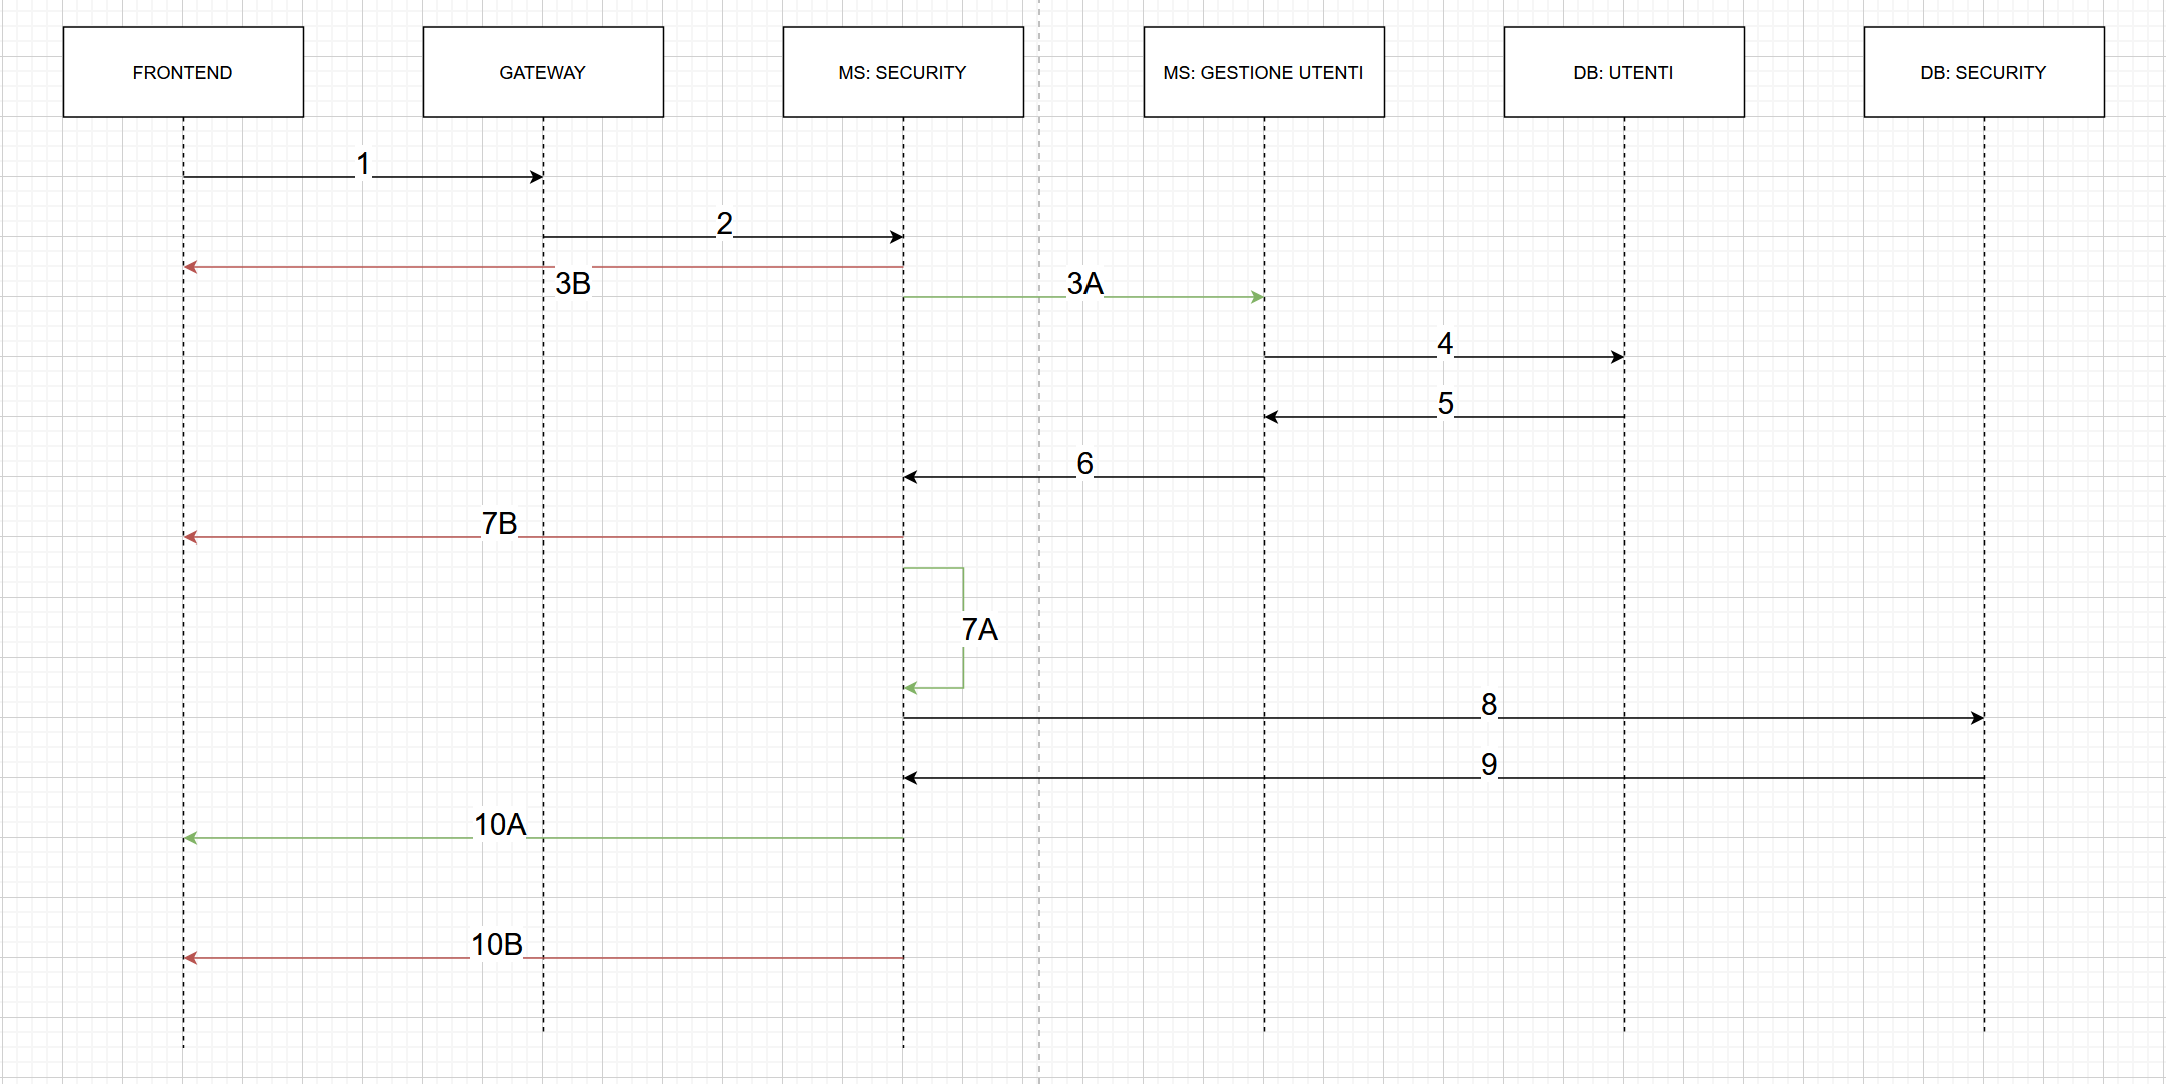
\includegraphics[width=450px, height=250px]{./images/registrazione.png}
        \caption{Flusso di registrazione}
        \label{fig:Registration}
    \end{figure}
\end{center}

\begin{itemize}
    \item[1.] Un utente con privilegi elevati può fare una richiesta di aggiunta  di un utente, egli va ad inserire la mail dell'utente (nome.cognome@certimeter.it) nell'apposito spazio ed effettua la richiesta premendo il tasto "SUBMIT".
    \item[2.] La richiesta viene inoltrata dal gateway al microservizio di security che si occuperà di eseguire dei controlli riguardo alla struttura della mail passata in input.
    \begin{itemize}
        \item[3B.] Se la mail non è nome.cognome@certimeter.it viene reinviato un errore al frontend che visualizza l'errore a schermo.
        \item[3A.] Se la mail è ben formata viene passata al microservizio di gestione utenti.
    \end{itemize}
    \item[4.] Il microservizio di gestione utenti controlla se la mail è presente all'interno del database degli utenti.
    \item[5.] Il database invia la risposta al microservizio di gestione degli utenti.
    \item[6.] Il microservizio di gestione degli utenti risponde al microservizio di security
    \begin{itemize}
        \item[7B.] Se la mail era già presente all'interno del database viene reinviato un errore al frontend che visualizza un apposito messaggio.
        \item[7A.] Altrimenti viene mandata una mail all'indirizzo indicato contenente l'url dell'applicazione web e una password temporanea che l'utente dovrà utilizzare per il primo accesso.
    \end{itemize}
    \item[8.] Dopo che la mail per il primo accesso è stata inviata l'utente viene aggiunto all'interno del database di sicurezza per consentirgli di eseguire la login.
    \item[9.] Il database di sicurezza risponde al microservizio di security che rimanda un messaggio al frontend.
    \begin{itemize}
        \item[10A.] Se la mail dell'utente e la sua password sono state inserite correttamente all'interno del database di sicurezza viene visualizzato un messaggio di riuscita nel frontend.
        \item[10B.] Se non è stato possibile inserire l'utente all'interno del database di sicurezza verrà rilanciato un errore e verrà visualizzato un messaggio nel frontend.
    \end{itemize}
\end{itemize}

Il secondo flusso che andrò a considerare è quello di login.

\begin{center}
    \begin{figure}[h]
        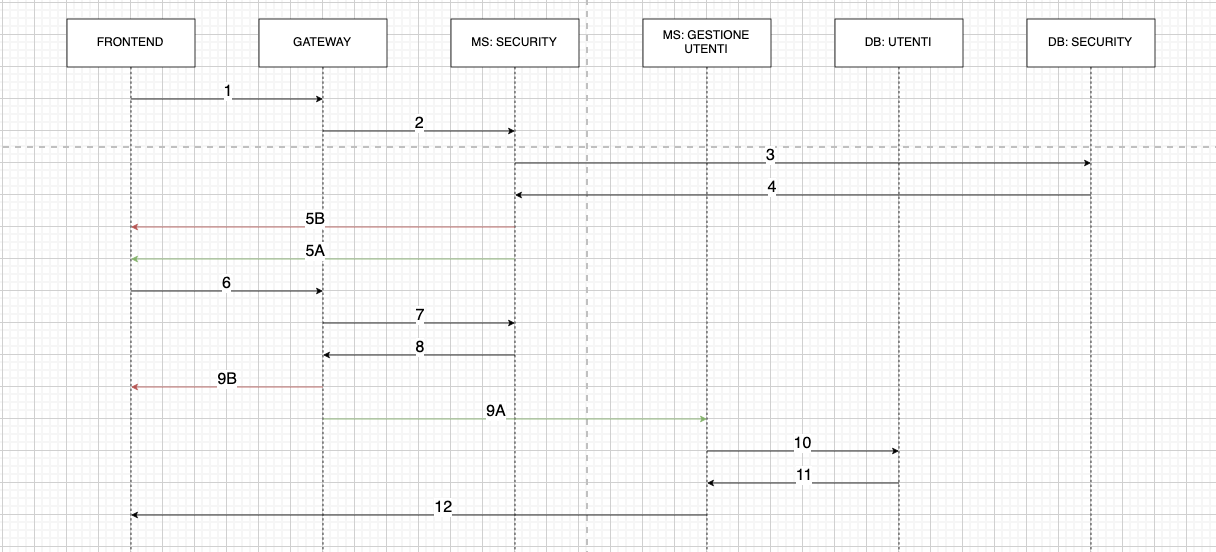
\includegraphics[width=450px, height=250px]{./images/flusso_login.png}
        \caption{Flusso di login}
        \label{fig:Registration}
    \end{figure}
\end{center}

Il flusso di login è più complicato di quanto non fosse inizialmente il caso d'uso associato perchè ho ritenuto importante far trasparire che a livello software la chiamata che richiede tutte le informazioni dell'utente avviene subito dopo che la richiesta di login è stata effettuata e convalidata.
\\
Detto questo passo ad esplicitare il significato del diagramma di flusso
\\
\begin{itemize}
    \item[1.] L'utente invia la richiesta al sistema inserendo email e password e premendo il pulsante di "SIGN IN".
    \item[2.] Il gateway reindirizza la richiesta al microservizio di sicurezza.
    \item[3.] Il microservizio di sicurezza confronta email e password con le entry presenti nel database di sicurezza.
    \item[4.] Il database inoltra la risposta al microservizio di sicurezza.
    \begin{itemize}
        \item[5B.] L'utente non è stato identificato all'interno del database, e quindi viene reinviato un errore al frontend (403), viene dunque visualizzato un messaggio a schermo.
        \item[5A.] \'E stata trovata una corrispondenza all'interno del database e quindi la login può essere eseguita, inizia il processo di reindirizzamento della sessione all'endpoint "/".
        \\
        Inoltre all'interno della risposta inviata dal backend è presente il token associato all'utente che contiene al suo interno una serie di informazioni criptate che possono essere utilizzate per riconoscerlo.
    \end{itemize}
    \item[6.] Il frontend manda al gateway la richiesta per tutti i dati dell'utente.
    \item[7.] Il gateway invia una prima richiesta di controllo del token al microservizio di sicurezza.
    \item[8.] Il microservizio di sicurezza esegue il controllo del token e rinvia il risultato al gateway.
    \begin{itemize}
        \item[9B.] Se il token non è stato convalidato il gateway rimanda un segnale di errore (403) al frontend e viene visualizzato a schermo un messaggio di errore.
        \item[9A.] Se il token viene invece convalidato la richiesta viene inoltrata dal gateway al microsevizio di gestione degli utenti.
    \end{itemize}
    \item[10.] Il microservizio di gestione invia la richiesta dei dati al database contenente i dati degli utenti.
    \item[11.] Il database risponde inviando il risultato della query.
    \item[12.] I dati vengono inviati in JSON al frontend che li visualizza all'interno della homepage
\end{itemize}

Come ultimo diagramma di sequenza si consideri il diagramma di sequenza di modifica degli attributi utente.

\begin{center}
    \begin{figure}[h]
        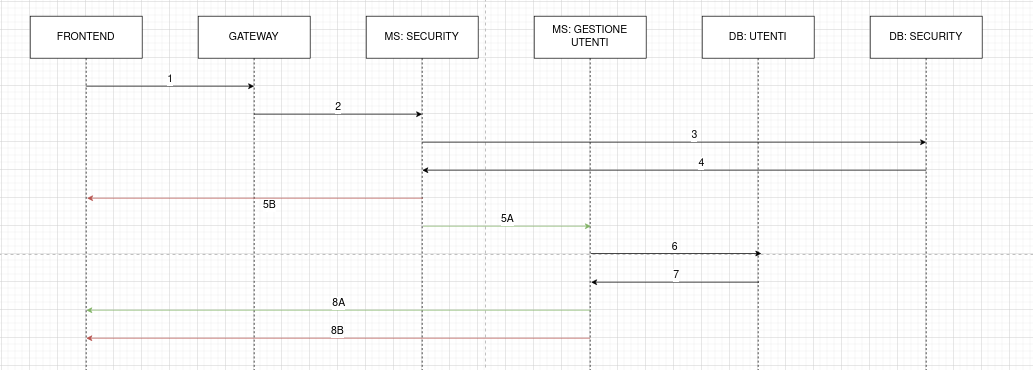
\includegraphics[width=450px, height=180px]{./images/attributi_utente.png}
        \caption{Flusso di modifica degli attributi utente}
        \label{fig:Registration}
    \end{figure}
\end{center}

\begin{itemize}
    \item[1.] Un utente cui sono associati privilegi di alto livello (admin o superAdmin), esegue una serie di aggiornamenti agli attributi di un utente, una volta terminato esegue la richiesta impiegando l'apposito bottone "SUBMIT". Una funzione invierà al backend il token dell'utente e le informazioni che ha modificato.
    \item[2.] La richiesta viene inoltrata dal gateway al microservizio di sicurezza che esegue un controllo sulla validità del token.
    \item[3.] I controlli vengono eseguiti rispetto ai dati contenuti nel database di security.
    \item[4.] Il database risponde alla query.
    \begin{itemize}
        \item[5B.] Se la risposta della query è negativa significa che il token non è stato riconosciuto o il token associato all'utente non ha i diritti necessari a poter eseguire l'operazione richiesta. Viene quindi restituito un (403) al frontend che visualizza a schermo un messaggio di errore.
        \item[5A.] Se la risposta della query è positiva allora si passa a sovrascrivere le informazioni, quindi vengono passate le modifiche al microservizio di gestione degli utenti.
    \end{itemize}
    \item[6.] Il microservizio di gestione utenti provvede a salvare le informazioni nel database.
    \item[7.] Il database risponde alla query.
    \begin{itemize}
        \item[8A.] Se non vi sono stati problemi durante il processo di aggiornamento viene inviato al frontend un messaggio di riuscita (200) e viene visualizzato a schermo un messaggio di conferma.
        \item[8B.] Se vi sono stati problemi durante l'aggiornamento viene reinviato al frontend un messaggio di errore (500) e viene visualizzato a schermo un messaggio di fallimento. 
    \end{itemize}
\end{itemize}



%%%%%%%%%%%%%%%%%%%%%%%%%%%%%
\section{Struttura a microservizi}
%%%%%%%%%%%%%%%%%%%%%%%%%%%%%
In questa sezione discuterò brevemente la struttura a microservizi dell'applicazione, uno schema può essere visto nella figura \ref{fig:microservices}.
\\
Nella mia configurazione ho incluso un firewall per proteggere la sottorete dall'esterno, il microservizio di gateway infatti filtra le richieste e blocca tutte quelle che non provengano dagli endpoint di frontend. Sarà poi il Gateway ad occuparsi di smistare le richieste tra i microservizi di gestione e di sec (o security).
\\
I due microservizi sono unità assolutamente indipendenti e separate, però necessitano di comunicare per poter portare a termine correttamente le operazioni richieste. Come si è visto in precedenza, per esempio, nel caso della registrazione, il microservizio di sicurezza esegue dei controlli sulla mail che viene passata in ingresso prima di inoltrarla al microservizio di gestione che si occuperà di notificare il candidato.
\\
Per ciascuno ho aggiunto un database separato e indipendente, in pieno rispetto delle norme di sviluppo a microservizi.

\begin{center}
    \begin{figure}[h]
        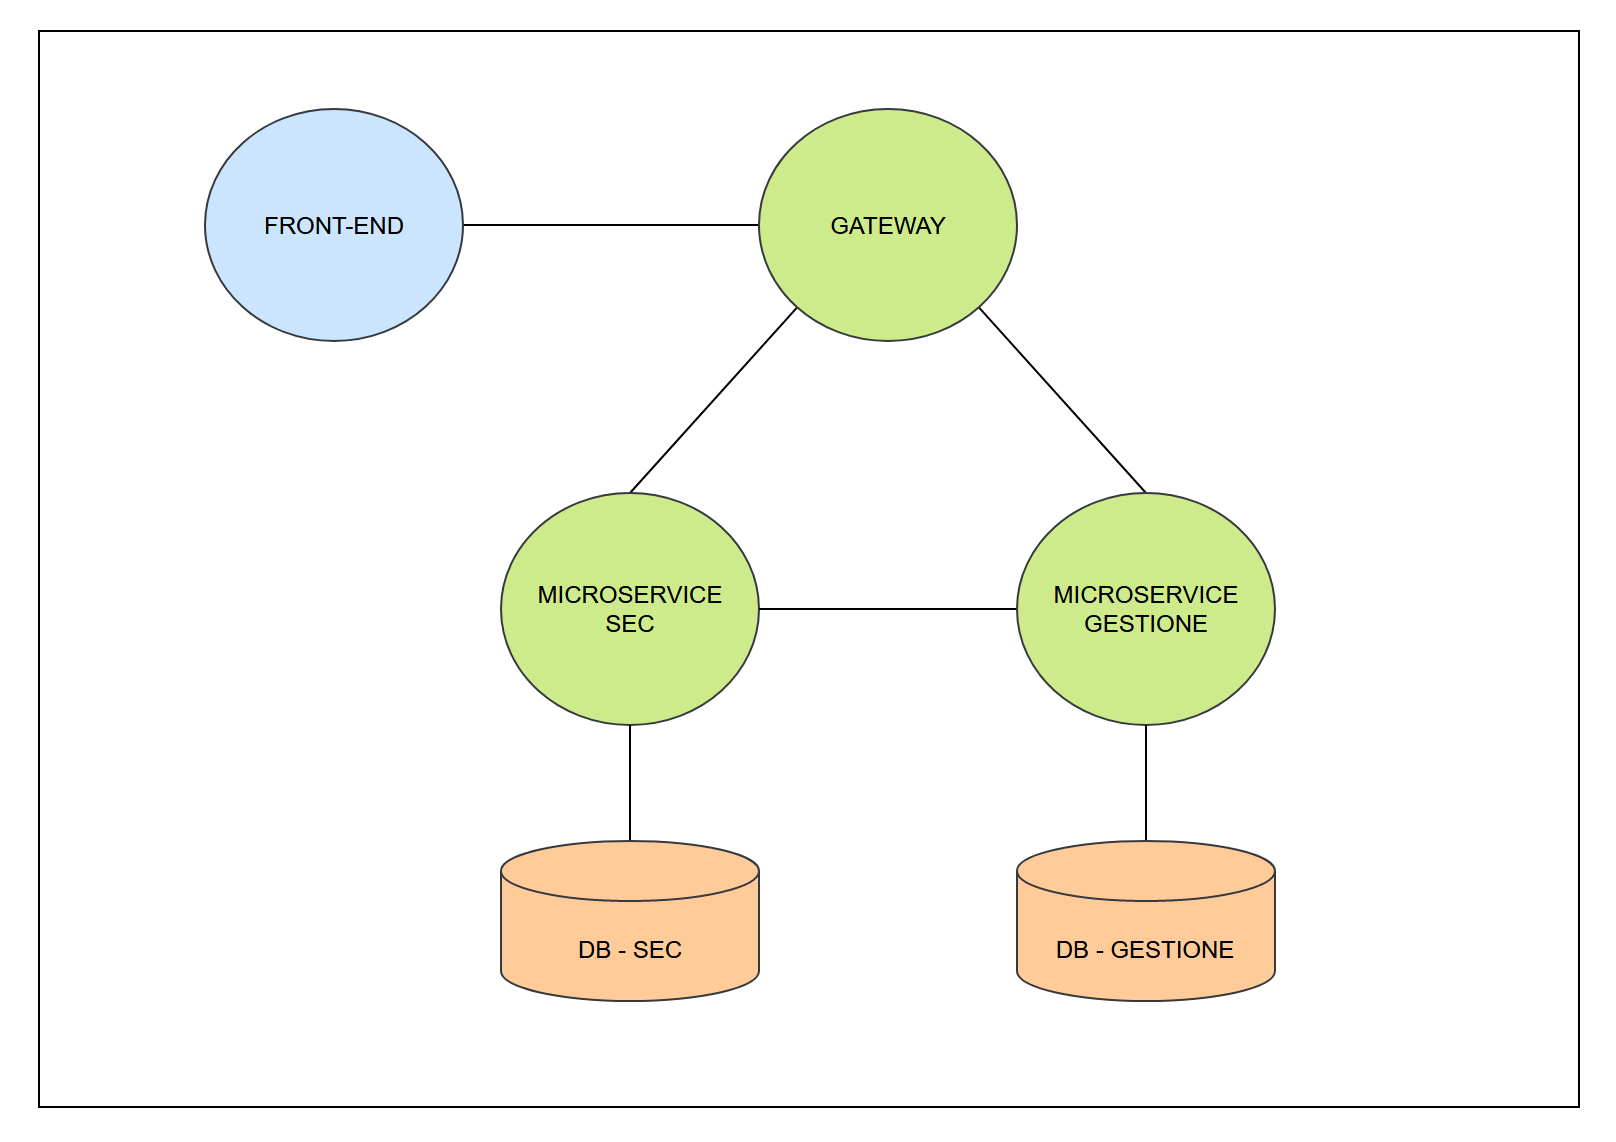
\includegraphics[width=450px]{./images/architettura.png}
        \caption{Architettura a microservizi}
        \label{fig:microservices}
    \end{figure}
\end{center}



%%%%%%%%%%%%%%%%%%%%%%%%%%%%%
\section{Database}
%%%%%%%%%%%%%%%%%%%%%%%%%%%%%
Per quel che riguarda i database, come si vedeva nella figura \ref{fig:microservices}, l'applicazione ne ha uno per la gestione della sicurezza, ed è sostanzialmente stato creato per gestire l'operazione di autenticazione e tutti controlli delle autorizzazioni tramite token.
\\
Il suo schema ER è quello che si può vedere nella figura \ref{security_db}.
\\
L'altro database contiene le informazioni di tutti gli utenti, la sua struttura è mostrata nella figura \ref{management_db}.
\\
Come si può vedere e com'è forse possibile intuire dai diagrammi di flusso esposti nella sezione precedente, sebbene i due database siano divisi non sono altro che due parti di un unico database che è stato diviso. Sarebbe infatti possibile legare l'entità ACCOUNT con l'entità PERSON per avere un database unico.
\begin{center}
    \begin{figure}
        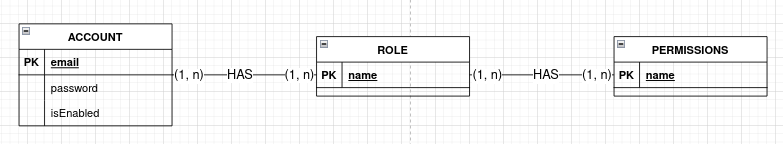
\includegraphics[width=450px]{./images/security_db.png}
        \caption{Schema relazionale per il database di sicurezza}
        \label{security_db}
    \end{figure}
\end{center}
\begin{center}
    \begin{figure}
        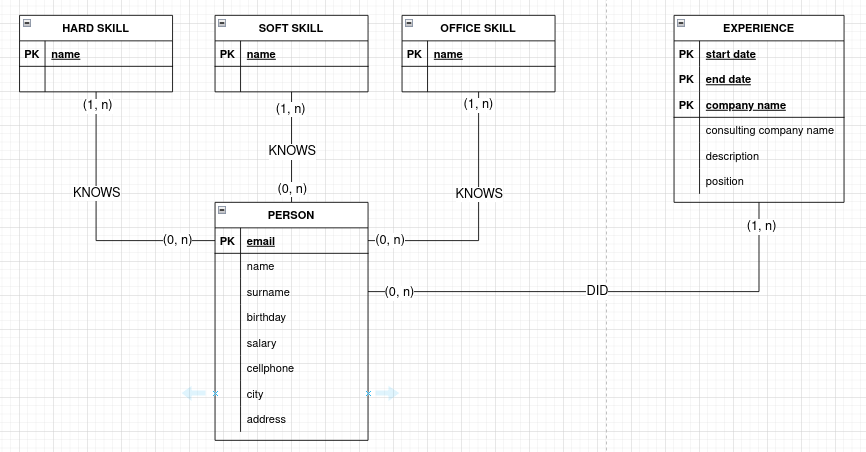
\includegraphics[width=450px]{./images/management_db.png}
        \caption{Schema relazionale per il database di management degli utenti}
        \label{management_db}
    \end{figure}
\end{center}